
%\newpage
\section{Selbsttest-Funktion}
\label{sec:selftest}
Beginnend mit Version 0.9k habe ich eine Selbsttest-Funktion eingebaut.
Die Benutzung ist sehr einfach.
Wenn Sie Prüfspitzen mit Klemmen verwenden, klemmen Sie alle Klemmen auf ein unisoliertes Stück Draht und drücken Sie
den Start-Taster.
Das Programm bemerkt die kurzgeschlossenen Klemmen und startet den Selbsttest.
Nach Beenden des Selbsttestes wird der Tester mit normaler Messung fortfahren.
Wenn kein Bauteil angeschlossen ist, wird der TransistorTester mit der
Meldung ,,kein,unbek. oder defektes Bauteil'' enden.
Man kann die Selbsttest-Funktion zusammen mit allen anderen Optionen nur für einen ATmega168
oder ATmega328 wählen.
Die einzelnen Schritte der Selbsttestfunktion werden für Test~1 bis Test~6 in Zeile~1 des LC-Displays mit dem Buchstaben T
gefolgt von der Schritt-Nummer dargestellt.
Die Schritte 1 bis 6 wird viermal wiederholt, bevor das Programm zum nächsten Schritt geht.
Aber wenn man den Start Taster gedrückt hält, wenn ein Durchlauf beendet wird, wird dieser Test nicht
mehr wiederholt.
Wenn man den Taster während dem gesamten Selbsttest gedrückt hält, wird jeder Schritt nur einmal ausgeführt.

Ohne die AUTO\_CAL Option werden in jedem Schritt nur Messergebnisse dargestellt, es wird keine Fehleranalyse durchgeführt.
Man  muss die Ergebnisse selbst interpretieren.
An dieser Stelle möchte ich noch einen wichtigen Hinweis geben. Führen Sie niemals Messungen mit
eingestecktem ISP-Stecker durch!
Die ISP-Schnittstelle st"ort die Messungen.

\vspace{1cm}
Hier ist die Liste der derzeit eingebauten Tests:
\vspace{1cm}
\begin{enumerate}
\item {\bf Messung der 1,3V (oder 1,1V) Referenzspannung (band gap Reference).} In Zeile~1 wird der Text ,,Ref='' und die
gemessene Spannung in mV angezeigt.
Für den ATmega8 sollte die gemessene Spannung nahe bei 1,3V liegen, für die anderen Prozessoren liegt
die Referenzspannung normal um die 1,1V.
Die zweite Zeile zeigt den resultierenden Faktor für die Kapazitäts-Messung mit dem \(470k\Omega\) Widerstand.
\item {\bf Vergleich der \(680\Omega\) Widerstände.} 
In Zeile~1 wird der kryptische Text  ,,+RL- 12 13 23'' angezeigt. Das bedeutet:
RL ist eine Kurzform für Resistor Low, was die \(680\Omega\) Widerstände meint. Die ,,12'' steht für: 
Widerstand am Pin~1 ist verbunden mit VCC (+) und Widerstand am Pin~2 ist verbunden mit GND (-). 
Das Ergebnis dieser Messung steht in Zeile~2 an erster Stelle als Differenz zum theoretischen Wert.
 In Zeile~1 folgt nun ,,13'', was bedeutet, dass der Widerstand von Pin~1 wieder nach VCC verbunden ist,
aber dass jetzt der \(680\Omega\) Widerstand von Pin~3  mit GND verbunden ist.
Das Ergebnis steht in Zeile 2 an der mittleren Stelle als Differenz zum theoretischen Wert.

Die letzte Messung dieses Tests ,,23'' bedeutet, dass nun der Widerstand von Pin~2 mit VCC verbunden ist und
der Widerstand von Pin~3 mit GND verbunden ist.
Das Ergebnis steht in der zweiten LCD-Zeile an letzter Stelle als Differenz zum theoretischen Wert.
Ich möchte daran erinnern, dass die Auflösung des ADC etwa 4,88mV beträgt!
Die Messsituation wird auch in Abbildung~\ref{fig:test2} dargestellt.
Der theoretische Wert ergibt sich im Hinblick auf die internen Port-Widerstände wie folgt:
\(\frac{5001 \cdot  (19+680)}{ (19+680+680+22)} = 2493\) .

\begin{figure}[H]
\centering

\includegraphics[width=17cm]{../FIG/Test2.eps}
\caption{Vergleich der \(680\Omega\)-Widerstände }
\label{fig:test2}
\end{figure}

\item {\bf Vergleich der \(470k\Omega\) Widerstände.}
Jetzt zeigt das Display in Zeile 1 ,,+RH- 12 13 23''. Das gleiche Verfahren wie in Schritt wird wiederholt mit den
 \(470k\Omega\)-Widerständen (Symbol RH).
Die Ergebnisse werden als Differenz zu  \(\frac{VCC \cdot (19 + 470000]}{ (19 + 470000 + 470000 + 22)} \) für alle Kombinationen dargestellt.
\item In diesem Schritt wird nichts gemessen, es erfolgt lediglich die {\bf Anweisung ,,isolate Probe''},
was bedeutet, dass es nun Zeit ist die Klemmen zu trennen (vom blanken Draht lösen).
\item Dieser Schritt testet die {\bf Fähigkeit von mit GND (-) verbundenen \(470k\Omega\)-Widerständen (H) die Testpins auf GND zu ziehen.}
Zeile 1 zeigt den Text ,,RH-''.
Zeile 2 sollte für alle drei Pinne  Null mV anzeigen.
\item Dieser Schritt testet die {\bf Fähigkeit von mit VCC (+) verbundenen \(470k\Omega\)-Widerständen (H) die Testpins auf VCC zu ziehen.}
Zeile 1 zeigt den Text ,,RH+''.
Der bestmögliche mV Wert für die drei Messungen wäre 0 in Zeile~2, da die Diffenz zu VCC dargestellt wird.
 große Abweichungen vom Idealwert für Schritt 5 und 6 sind Fehler wie Isolations-Problem, Flussmittelreste oder beschädigter Port.
\item {\bf Messung des Innenwiderstandes eines auf GND geschalteten Ausgangs.}
Dieser und die folgenden Schritte werden nur bei gewählter AUTO\_CAL Option durchgeführt.
Die internen Port C Widerstände von auf GND (-) geschalteten Ausgängen werden mit dem Strom
der nach VCC (+) geschalteten \(680\Omega\) Widerstände gemessen, siehe Abbildung~\ref{fig:test7}.
Es werden nur die drei Pins des ADC-Ports vermessen, die Widerstands-Ports  PB0, PB2 und PB4 können nicht
ohne Veränderung der Hardware gemessen werden.
Es wird angenommen, dass die Portwiderstände von unterschiedlichen Ports nahezu identisch sind.
Der Widerstandswert wird im nächsten Schritt mit ausgegeben.
\begin{figure}[H]
\centering

\includegraphics[]{../FIG/Test7.eps}
\caption{Messung des Innenwiderstandes von auf GND geschalteten Port-C-Ausgängen.}
\label{fig:test7}
\end{figure}

\item {\bf Messung des Innenwiderstandes von auf VCC geschalteten Port-Ausgängen.}
Der benötigte Strom wird von auf GND geschalteten \(680\Omega\)-Widerständen geliefert.
Es ist die gleiche Messung wie die in Test~7 zur anderen Seite, wie in Abbildung \ref{fig:test8} gezeigt wird.
Der Innenwiderstand wird wie folgt berechnet:
Um den Strom zu berechnen: \((5001 - (Ergebnis von Test 7) - (Ergebnis von Test 8)) / 680\).
Die Widerstandswerte ergeben sich, wenn die gemessene Spannung durch diesen Strom dividiert wird.
Der gefundene Mittelwert der Innenwiderstände der Ausgabe-Ports wird im EEprom festgehalten.
Das Ergebnis für diesen Test wird dann in Zeile~1 mit dem Text ,,RI\_Hi=''in \(\Omega\) angezeigt, der Innenwiderstand
zur GND-Seite wird in Zeile~2 mit dem Text ,,RI\_Lo='' angezeigt.
Diese Werte stehen dann für weitere Messungen zur Verfügung.
\begin{figure}[H]
\centering

\includegraphics[]{../FIG/Test8.eps}
\caption{Messung des Innenwiderstandes des auf VCC geschalteten Port-C-Ausgängen.}
\label{fig:test8}
\end{figure}

\item {\bf Messung des Nulloffsets der Kondensatormessung.}
Für die Pinkombinationen 1:3, 2:3 und 1:2 wird der Nullwert der Kondensatormessung in pF ausgegeben.
In der Software wird ein Vorgabewert von circa 39~pF für die normale Messwertausgabe berücksichtigt.
Für die Ausgabe dieses Tests ist keine Korrektur berücksichtigt, es wird auch kein Nulloffset abgezogen.
Die gefundenen Nulloffsets werden im EEprom festgehalten, wenn alle Null Offsets kleiner als 70pF sind.
Die gefundene Null Offsets werden für die weiteren Kapazitäts-Messungen Pin abhängig berücksichtigt.
Angezeigt wird  die Ausgabe ,,C0''  in Zeile 1, gefolgt von den drei Null-Offsets für
die Pin-Kombinationen 1:3, 2:3 und 1:2 .
Bitte beachten Sie, dass Veränderungen des Messaufbaus einen Neuabgleich sinnvoll machen.
So kann sich der Nulloffset durch Verwenden von Kabeln mit Klemmen um circa 3~pF gegenüber einem leeren
Sockel erhöhen.

\item {\bf Warten auf den Anschluss eines Kondensators an Pin~1 und Pin~3.}
Zur Vorbereitung der Messung des Spannungs-Offsets des analogen Komparators muss ein ausreichend großer
Kondensator zwischen Pin 1 und Pin 3 angeschlossen werden.
Es sollte ein Kondensator hoher Güte mit eine Kapazität zwischen \(100 nF\) und \(20 \mu F\) sein. 
Auf keinen Fall sollte man Elektrolyt-Kondensatoren verwenden.


\item {\bf Messung des Komparatoroffsets für den Abgleich der Kondensatormessung.}
Um den Offset des analogen Komparators zu bestimmen, muss ein Kondensator an Pin~1 und Pin~3 angeschlossen sein.
Der Kondensator wird für die Pufferung der Ladespannung bei der Kondensatormessung benötigt, um den Unterschied der 
Ladespannung zur internen Referenzspannung bestimmen zu können.
Bei erfolgreicher Messung wird der Korrekturwert kurz in Zeile 1 mit dem Text ,,REF\_C='' angezeigt und in den EEprom-Speicher geschrieben.
Wenn Sie die AUTOSCALE\_ADC-Option gewählt haben, wird die Verstärkung der ADC-Lesefunktion mit der
internen Referenzspannung abgeglichen. Das geschieht durch den Vergleich der Kondensatorspannung von unter 1 V, einmal mit
der VCC-Referenz gemessen und einmal mit der internen Referenz.
Die gefundene Differenz wird in Zeile 2 mit dem Text ,,REF\_R='' angezeigt und ebenfalls im EEprom festgehalten.
Der REF\_R\_KORR-Wert ist dann nur ein zusätzlicher Offset f\"r diese automatisch gefundene Differenz.

\end{enumerate}

An Ende der Selbsttest-Funktion wird der Text ,,Auto Test End'' in Zeile~1 und die Versions-Nummer der Software in Zeile~2 angezeigt.
Wenn gewählt, wird ein {\bf 50 Hz Rechtecksignal} auf Testpin~2 generiert und das gegenphasige Signal auf Testpin~3.
Testpin~1 wird auf GND geschaltet. Der Strom für Testpin 2 und 3 wird mit \(680\Omega\) Widerständen begrenzt.
Angezeigt wird das durch die Ausgabe von ''50Hz'' am Ende der Zeile~1.
Diese Ausgabe wird dreißig Mal mit jeweils 2~Sekunden Dauer durchgeführt.
Man kann die Zeit der Verzögerungs-Aufrufe prüfen, wenn man ein Oszilloskop oder einen
Frequenz-Zähler besitzt.
Wenn man für die Takterzeugung keinen Quarz benutzt, können die
Ergebnisse der Kondensatormessung ungenau sein.
Eine genaue Taktfrequenz und genaue Wartezeiten sind wichtig für die Bestimmung von Kapazitätswerten.
Die Ausgabe des 50Hz-Signals kann durch Gedrückthalten des Start-Tasters vorzeitig abgebrochen werden.
Dann fährt das Programm mit der normalen Messfunktion fort.


Die Ergebnisse des Selbsttests der 9 verschiedenen ATmega168-Prozessoren und der 6 ATmega328-Prozessoren
sind in den folgenden Abbildungen dargestellt. 

\begin{table}[H]
  \begin{center}
    \begin{tabular}{| l | c | c | c |}
    \hline
Test No. &  Messtyp    & Idealwert & Abbildung \\
    \hline
    \hline
Test 1 & band gap Ref  & 1100 & \ref{fig:SelfTref} \\
    \hline
Test 2 & RL Mitte & 0 & \ref{fig:SelfTMitL} \\
    \hline
Test 3 & RH Mitte & 0 & \ref{fig:SelfTMitH} \\
    \hline
Test 5 & RH Low &  0 & \ref{fig:SelfTlowH} \\
    \hline
Test 6 & RH High & 0 & \ref{fig:SelfTtopH} \\
    \hline
Test 7 & R out Lo & 131 & \ref{fig:SelfTRoL} \\
    \hline
Test 8 & R out Hi & 151 & \ref{fig:SelfTRoH} \\
    \hline
Test 9 & Cap0  & 30 & \ref{fig:SelfTcap} \\
    \hline
Test 9 & Referenz-Korrektur  & 0 & \ref{fig:SelfTrefKorr} \\
    \hline
    \end{tabular}
  \end{center}
  \caption{Verzeichnis der Selbsttest-Diagramme}
  \label{tab:test_m168} 
\end{table}

\begin{figure}[H]
  \centering
  % GNUPLOT: LaTeX picture with Postscript
\begingroup
  \makeatletter
  \providecommand\color[2][]{%
    \GenericError{(gnuplot) \space\space\space\@spaces}{%
      Package color not loaded in conjunction with
      terminal option `colourtext'%
    }{See the gnuplot documentation for explanation.%
    }{Either use 'blacktext' in gnuplot or load the package
      color.sty in LaTeX.}%
    \renewcommand\color[2][]{}%
  }%
  \providecommand\includegraphics[2][]{%
    \GenericError{(gnuplot) \space\space\space\@spaces}{%
      Package graphicx or graphics not loaded%
    }{See the gnuplot documentation for explanation.%
    }{The gnuplot epslatex terminal needs graphicx.sty or graphics.sty.}%
    \renewcommand\includegraphics[2][]{}%
  }%
  \providecommand\rotatebox[2]{#2}%
  \@ifundefined{ifGPcolor}{%
    \newif\ifGPcolor
    \GPcolortrue
  }{}%
  \@ifundefined{ifGPblacktext}{%
    \newif\ifGPblacktext
    \GPblacktexttrue
  }{}%
  % define a \g@addto@macro without @ in the name:
  \let\gplgaddtomacro\g@addto@macro
  % define empty templates for all commands taking text:
  \gdef\gplbacktext{}%
  \gdef\gplfronttext{}%
  \makeatother
  \ifGPblacktext
    % no textcolor at all
    \def\colorrgb#1{}%
    \def\colorgray#1{}%
  \else
    % gray or color?
    \ifGPcolor
      \def\colorrgb#1{\color[rgb]{#1}}%
      \def\colorgray#1{\color[gray]{#1}}%
      \expandafter\def\csname LTw\endcsname{\color{white}}%
      \expandafter\def\csname LTb\endcsname{\color{black}}%
      \expandafter\def\csname LTa\endcsname{\color{black}}%
      \expandafter\def\csname LT0\endcsname{\color[rgb]{1,0,0}}%
      \expandafter\def\csname LT1\endcsname{\color[rgb]{0,1,0}}%
      \expandafter\def\csname LT2\endcsname{\color[rgb]{0,0,1}}%
      \expandafter\def\csname LT3\endcsname{\color[rgb]{1,0,1}}%
      \expandafter\def\csname LT4\endcsname{\color[rgb]{0,1,1}}%
      \expandafter\def\csname LT5\endcsname{\color[rgb]{1,1,0}}%
      \expandafter\def\csname LT6\endcsname{\color[rgb]{0,0,0}}%
      \expandafter\def\csname LT7\endcsname{\color[rgb]{1,0.3,0}}%
      \expandafter\def\csname LT8\endcsname{\color[rgb]{0.5,0.5,0.5}}%
    \else
      % gray
      \def\colorrgb#1{\color{black}}%
      \def\colorgray#1{\color[gray]{#1}}%
      \expandafter\def\csname LTw\endcsname{\color{white}}%
      \expandafter\def\csname LTb\endcsname{\color{black}}%
      \expandafter\def\csname LTa\endcsname{\color{black}}%
      \expandafter\def\csname LT0\endcsname{\color{black}}%
      \expandafter\def\csname LT1\endcsname{\color{black}}%
      \expandafter\def\csname LT2\endcsname{\color{black}}%
      \expandafter\def\csname LT3\endcsname{\color{black}}%
      \expandafter\def\csname LT4\endcsname{\color{black}}%
      \expandafter\def\csname LT5\endcsname{\color{black}}%
      \expandafter\def\csname LT6\endcsname{\color{black}}%
      \expandafter\def\csname LT7\endcsname{\color{black}}%
      \expandafter\def\csname LT8\endcsname{\color{black}}%
    \fi
  \fi
  \setlength{\unitlength}{0.0500bp}%
  \begin{picture}(7200.00,5040.00)%
    \gplgaddtomacro\gplbacktext{%
      \csname LTb\endcsname%
      \put(1078,704){\makebox(0,0)[r]{\strut{} 1050}}%
      \csname LTb\endcsname%
      \put(1078,1383){\makebox(0,0)[r]{\strut{} 1060}}%
      \csname LTb\endcsname%
      \put(1078,2061){\makebox(0,0)[r]{\strut{} 1070}}%
      \csname LTb\endcsname%
      \put(1078,2740){\makebox(0,0)[r]{\strut{} 1080}}%
      \csname LTb\endcsname%
      \put(1078,3418){\makebox(0,0)[r]{\strut{} 1090}}%
      \csname LTb\endcsname%
      \put(1078,4097){\makebox(0,0)[r]{\strut{} 1100}}%
      \csname LTb\endcsname%
      \put(1078,4775){\makebox(0,0)[r]{\strut{} 1110}}%
      \csname LTb\endcsname%
      \put(1210,484){\makebox(0,0){\strut{} 0}}%
      \csname LTb\endcsname%
      \put(1560,484){\makebox(0,0){\strut{} 1}}%
      \csname LTb\endcsname%
      \put(1909,484){\makebox(0,0){\strut{} 2}}%
      \csname LTb\endcsname%
      \put(2259,484){\makebox(0,0){\strut{} 3}}%
      \csname LTb\endcsname%
      \put(2608,484){\makebox(0,0){\strut{} 4}}%
      \csname LTb\endcsname%
      \put(2958,484){\makebox(0,0){\strut{} 5}}%
      \csname LTb\endcsname%
      \put(3307,484){\makebox(0,0){\strut{} 6}}%
      \csname LTb\endcsname%
      \put(3657,484){\makebox(0,0){\strut{} 7}}%
      \csname LTb\endcsname%
      \put(4007,484){\makebox(0,0){\strut{} 8}}%
      \csname LTb\endcsname%
      \put(4356,484){\makebox(0,0){\strut{} 9}}%
      \csname LTb\endcsname%
      \put(4706,484){\makebox(0,0){\strut{} 10}}%
      \csname LTb\endcsname%
      \put(5055,484){\makebox(0,0){\strut{} 11}}%
      \csname LTb\endcsname%
      \put(5405,484){\makebox(0,0){\strut{} 12}}%
      \csname LTb\endcsname%
      \put(5754,484){\makebox(0,0){\strut{} 13}}%
      \csname LTb\endcsname%
      \put(6104,484){\makebox(0,0){\strut{} 14}}%
      \csname LTb\endcsname%
      \put(6453,484){\makebox(0,0){\strut{} 15}}%
      \csname LTb\endcsname%
      \put(6803,484){\makebox(0,0){\strut{} 16}}%
      \put(176,2739){\rotatebox{-270}{\makebox(0,0){\strut{}reference voltage / mV}}}%
      \put(4006,154){\makebox(0,0){\strut{}Processor number}}%
      \put(4006,4665){\makebox(0,0){\strut{}}}%
    }%
    \gplgaddtomacro\gplfronttext{%
      \csname LTb\endcsname%
      \put(5690,4594){\makebox(0,0)[r]{\strut{}Reference}}%
    }%
    \gplbacktext
    \put(0,0){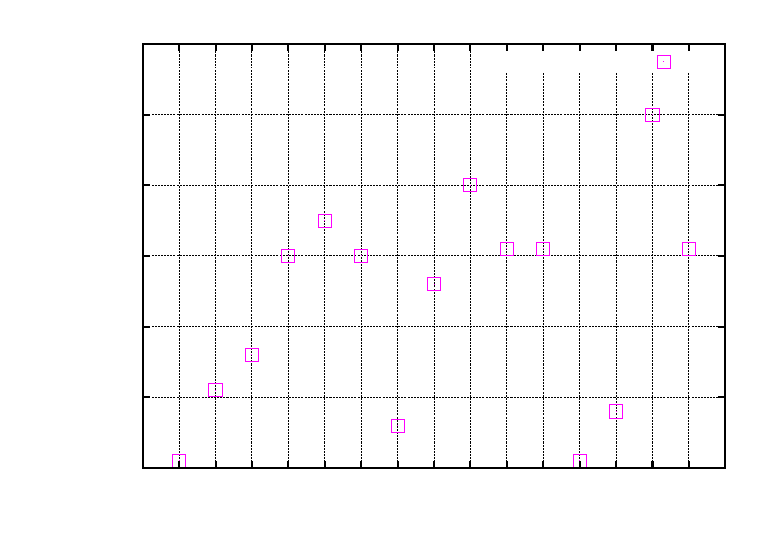
\includegraphics{../GNU/SelfTref}}%
    \gplfronttext
  \end{picture}%
\endgroup

  \caption{Selbsttest: Referenz-Spannungen}
  \label{fig:SelfTref}
\end{figure}

\begin{figure}[H]
  \begin{subfigure}[b]{9cm}
    \centering
    \resizebox{9cm}{!}{% GNUPLOT: LaTeX picture with Postscript
\begingroup
  \makeatletter
  \providecommand\color[2][]{%
    \GenericError{(gnuplot) \space\space\space\@spaces}{%
      Package color not loaded in conjunction with
      terminal option `colourtext'%
    }{See the gnuplot documentation for explanation.%
    }{Either use 'blacktext' in gnuplot or load the package
      color.sty in LaTeX.}%
    \renewcommand\color[2][]{}%
  }%
  \providecommand\includegraphics[2][]{%
    \GenericError{(gnuplot) \space\space\space\@spaces}{%
      Package graphicx or graphics not loaded%
    }{See the gnuplot documentation for explanation.%
    }{The gnuplot epslatex terminal needs graphicx.sty or graphics.sty.}%
    \renewcommand\includegraphics[2][]{}%
  }%
  \providecommand\rotatebox[2]{#2}%
  \@ifundefined{ifGPcolor}{%
    \newif\ifGPcolor
    \GPcolortrue
  }{}%
  \@ifundefined{ifGPblacktext}{%
    \newif\ifGPblacktext
    \GPblacktexttrue
  }{}%
  % define a \g@addto@macro without @ in the name:
  \let\gplgaddtomacro\g@addto@macro
  % define empty templates for all commands taking text:
  \gdef\gplbacktext{}%
  \gdef\gplfronttext{}%
  \makeatother
  \ifGPblacktext
    % no textcolor at all
    \def\colorrgb#1{}%
    \def\colorgray#1{}%
  \else
    % gray or color?
    \ifGPcolor
      \def\colorrgb#1{\color[rgb]{#1}}%
      \def\colorgray#1{\color[gray]{#1}}%
      \expandafter\def\csname LTw\endcsname{\color{white}}%
      \expandafter\def\csname LTb\endcsname{\color{black}}%
      \expandafter\def\csname LTa\endcsname{\color{black}}%
      \expandafter\def\csname LT0\endcsname{\color[rgb]{1,0,0}}%
      \expandafter\def\csname LT1\endcsname{\color[rgb]{0,1,0}}%
      \expandafter\def\csname LT2\endcsname{\color[rgb]{0,0,1}}%
      \expandafter\def\csname LT3\endcsname{\color[rgb]{1,0,1}}%
      \expandafter\def\csname LT4\endcsname{\color[rgb]{0,1,1}}%
      \expandafter\def\csname LT5\endcsname{\color[rgb]{1,1,0}}%
      \expandafter\def\csname LT6\endcsname{\color[rgb]{0,0,0}}%
      \expandafter\def\csname LT7\endcsname{\color[rgb]{1,0.3,0}}%
      \expandafter\def\csname LT8\endcsname{\color[rgb]{0.5,0.5,0.5}}%
    \else
      % gray
      \def\colorrgb#1{\color{black}}%
      \def\colorgray#1{\color[gray]{#1}}%
      \expandafter\def\csname LTw\endcsname{\color{white}}%
      \expandafter\def\csname LTb\endcsname{\color{black}}%
      \expandafter\def\csname LTa\endcsname{\color{black}}%
      \expandafter\def\csname LT0\endcsname{\color{black}}%
      \expandafter\def\csname LT1\endcsname{\color{black}}%
      \expandafter\def\csname LT2\endcsname{\color{black}}%
      \expandafter\def\csname LT3\endcsname{\color{black}}%
      \expandafter\def\csname LT4\endcsname{\color{black}}%
      \expandafter\def\csname LT5\endcsname{\color{black}}%
      \expandafter\def\csname LT6\endcsname{\color{black}}%
      \expandafter\def\csname LT7\endcsname{\color{black}}%
      \expandafter\def\csname LT8\endcsname{\color{black}}%
    \fi
  \fi
  \setlength{\unitlength}{0.0500bp}%
  \begin{picture}(7200.00,5040.00)%
    \gplgaddtomacro\gplbacktext{%
      \csname LTb\endcsname%
      \put(1078,704){\makebox(0,0)[r]{\strut{} 2480}}%
      \csname LTb\endcsname%
      \put(1078,1518){\makebox(0,0)[r]{\strut{} 2485}}%
      \csname LTb\endcsname%
      \put(1078,2332){\makebox(0,0)[r]{\strut{} 2490}}%
      \csname LTb\endcsname%
      \put(1078,3147){\makebox(0,0)[r]{\strut{} 2495}}%
      \csname LTb\endcsname%
      \put(1078,3961){\makebox(0,0)[r]{\strut{} 2500}}%
      \csname LTb\endcsname%
      \put(1078,4775){\makebox(0,0)[r]{\strut{} 2505}}%
      \csname LTb\endcsname%
      \put(1210,484){\makebox(0,0){\strut{} 0}}%
      \csname LTb\endcsname%
      \put(1560,484){\makebox(0,0){\strut{} 1}}%
      \csname LTb\endcsname%
      \put(1909,484){\makebox(0,0){\strut{} 2}}%
      \csname LTb\endcsname%
      \put(2259,484){\makebox(0,0){\strut{} 3}}%
      \csname LTb\endcsname%
      \put(2608,484){\makebox(0,0){\strut{} 4}}%
      \csname LTb\endcsname%
      \put(2958,484){\makebox(0,0){\strut{} 5}}%
      \csname LTb\endcsname%
      \put(3307,484){\makebox(0,0){\strut{} 6}}%
      \csname LTb\endcsname%
      \put(3657,484){\makebox(0,0){\strut{} 7}}%
      \csname LTb\endcsname%
      \put(4007,484){\makebox(0,0){\strut{} 8}}%
      \csname LTb\endcsname%
      \put(4356,484){\makebox(0,0){\strut{} 9}}%
      \csname LTb\endcsname%
      \put(4706,484){\makebox(0,0){\strut{} 10}}%
      \csname LTb\endcsname%
      \put(5055,484){\makebox(0,0){\strut{} 11}}%
      \csname LTb\endcsname%
      \put(5405,484){\makebox(0,0){\strut{} 12}}%
      \csname LTb\endcsname%
      \put(5754,484){\makebox(0,0){\strut{} 13}}%
      \csname LTb\endcsname%
      \put(6104,484){\makebox(0,0){\strut{} 14}}%
      \csname LTb\endcsname%
      \put(6453,484){\makebox(0,0){\strut{} 15}}%
      \csname LTb\endcsname%
      \put(6803,484){\makebox(0,0){\strut{} 16}}%
      \put(176,2739){\rotatebox{-270}{\makebox(0,0){\strut{}voltage / mV}}}%
      \put(4006,154){\makebox(0,0){\strut{}Processor number}}%
      \put(4006,4665){\makebox(0,0){\strut{}}}%
    }%
    \gplgaddtomacro\gplfronttext{%
      \csname LTb\endcsname%
      \put(5753,4602){\makebox(0,0)[r]{\strut{}RLmiddle12}}%
      \csname LTb\endcsname%
      \put(5753,4382){\makebox(0,0)[r]{\strut{}RLmiddle13}}%
      \csname LTb\endcsname%
      \put(5753,4162){\makebox(0,0)[r]{\strut{}RLmiddle23}}%
    }%
    \gplbacktext
    \put(0,0){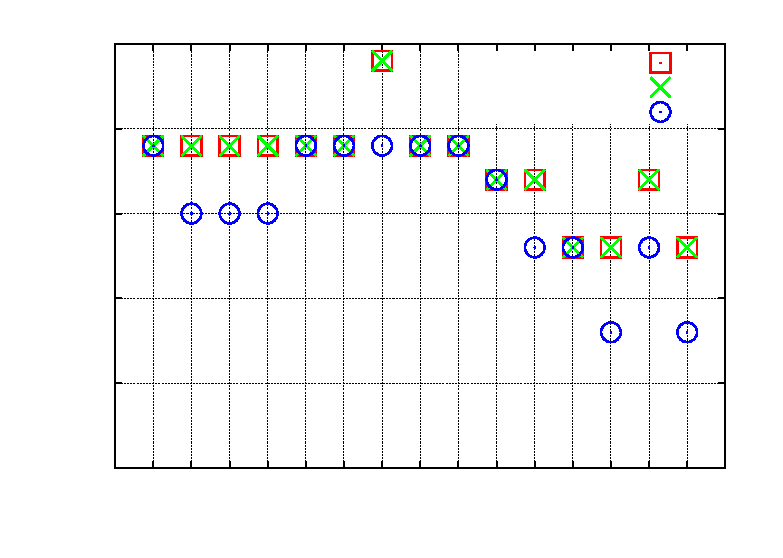
\includegraphics{../GNU/SelfTMitL}}%
    \gplfronttext
  \end{picture}%
\endgroup
}
    \caption{mit \(680 \Omega\)}
    \label{fig:SelfTMitL}
  \end{subfigure}
  ~
  \begin{subfigure}[b]{9cm}
    \centering
    \resizebox{9cm}{!}{% GNUPLOT: LaTeX picture with Postscript
\begingroup
  \makeatletter
  \providecommand\color[2][]{%
    \GenericError{(gnuplot) \space\space\space\@spaces}{%
      Package color not loaded in conjunction with
      terminal option `colourtext'%
    }{See the gnuplot documentation for explanation.%
    }{Either use 'blacktext' in gnuplot or load the package
      color.sty in LaTeX.}%
    \renewcommand\color[2][]{}%
  }%
  \providecommand\includegraphics[2][]{%
    \GenericError{(gnuplot) \space\space\space\@spaces}{%
      Package graphicx or graphics not loaded%
    }{See the gnuplot documentation for explanation.%
    }{The gnuplot epslatex terminal needs graphicx.sty or graphics.sty.}%
    \renewcommand\includegraphics[2][]{}%
  }%
  \providecommand\rotatebox[2]{#2}%
  \@ifundefined{ifGPcolor}{%
    \newif\ifGPcolor
    \GPcolortrue
  }{}%
  \@ifundefined{ifGPblacktext}{%
    \newif\ifGPblacktext
    \GPblacktexttrue
  }{}%
  % define a \g@addto@macro without @ in the name:
  \let\gplgaddtomacro\g@addto@macro
  % define empty templates for all commands taking text:
  \gdef\gplbacktext{}%
  \gdef\gplfronttext{}%
  \makeatother
  \ifGPblacktext
    % no textcolor at all
    \def\colorrgb#1{}%
    \def\colorgray#1{}%
  \else
    % gray or color?
    \ifGPcolor
      \def\colorrgb#1{\color[rgb]{#1}}%
      \def\colorgray#1{\color[gray]{#1}}%
      \expandafter\def\csname LTw\endcsname{\color{white}}%
      \expandafter\def\csname LTb\endcsname{\color{black}}%
      \expandafter\def\csname LTa\endcsname{\color{black}}%
      \expandafter\def\csname LT0\endcsname{\color[rgb]{1,0,0}}%
      \expandafter\def\csname LT1\endcsname{\color[rgb]{0,1,0}}%
      \expandafter\def\csname LT2\endcsname{\color[rgb]{0,0,1}}%
      \expandafter\def\csname LT3\endcsname{\color[rgb]{1,0,1}}%
      \expandafter\def\csname LT4\endcsname{\color[rgb]{0,1,1}}%
      \expandafter\def\csname LT5\endcsname{\color[rgb]{1,1,0}}%
      \expandafter\def\csname LT6\endcsname{\color[rgb]{0,0,0}}%
      \expandafter\def\csname LT7\endcsname{\color[rgb]{1,0.3,0}}%
      \expandafter\def\csname LT8\endcsname{\color[rgb]{0.5,0.5,0.5}}%
    \else
      % gray
      \def\colorrgb#1{\color{black}}%
      \def\colorgray#1{\color[gray]{#1}}%
      \expandafter\def\csname LTw\endcsname{\color{white}}%
      \expandafter\def\csname LTb\endcsname{\color{black}}%
      \expandafter\def\csname LTa\endcsname{\color{black}}%
      \expandafter\def\csname LT0\endcsname{\color{black}}%
      \expandafter\def\csname LT1\endcsname{\color{black}}%
      \expandafter\def\csname LT2\endcsname{\color{black}}%
      \expandafter\def\csname LT3\endcsname{\color{black}}%
      \expandafter\def\csname LT4\endcsname{\color{black}}%
      \expandafter\def\csname LT5\endcsname{\color{black}}%
      \expandafter\def\csname LT6\endcsname{\color{black}}%
      \expandafter\def\csname LT7\endcsname{\color{black}}%
      \expandafter\def\csname LT8\endcsname{\color{black}}%
    \fi
  \fi
  \setlength{\unitlength}{0.0500bp}%
  \begin{picture}(7200.00,5040.00)%
    \gplgaddtomacro\gplbacktext{%
      \csname LTb\endcsname%
      \put(1078,704){\makebox(0,0)[r]{\strut{} 2480}}%
      \csname LTb\endcsname%
      \put(1078,1518){\makebox(0,0)[r]{\strut{} 2485}}%
      \csname LTb\endcsname%
      \put(1078,2332){\makebox(0,0)[r]{\strut{} 2490}}%
      \csname LTb\endcsname%
      \put(1078,3147){\makebox(0,0)[r]{\strut{} 2495}}%
      \csname LTb\endcsname%
      \put(1078,3961){\makebox(0,0)[r]{\strut{} 2500}}%
      \csname LTb\endcsname%
      \put(1078,4775){\makebox(0,0)[r]{\strut{} 2505}}%
      \csname LTb\endcsname%
      \put(1210,484){\makebox(0,0){\strut{} 0}}%
      \csname LTb\endcsname%
      \put(1560,484){\makebox(0,0){\strut{} 1}}%
      \csname LTb\endcsname%
      \put(1909,484){\makebox(0,0){\strut{} 2}}%
      \csname LTb\endcsname%
      \put(2259,484){\makebox(0,0){\strut{} 3}}%
      \csname LTb\endcsname%
      \put(2608,484){\makebox(0,0){\strut{} 4}}%
      \csname LTb\endcsname%
      \put(2958,484){\makebox(0,0){\strut{} 5}}%
      \csname LTb\endcsname%
      \put(3307,484){\makebox(0,0){\strut{} 6}}%
      \csname LTb\endcsname%
      \put(3657,484){\makebox(0,0){\strut{} 7}}%
      \csname LTb\endcsname%
      \put(4007,484){\makebox(0,0){\strut{} 8}}%
      \csname LTb\endcsname%
      \put(4356,484){\makebox(0,0){\strut{} 9}}%
      \csname LTb\endcsname%
      \put(4706,484){\makebox(0,0){\strut{} 10}}%
      \csname LTb\endcsname%
      \put(5055,484){\makebox(0,0){\strut{} 11}}%
      \csname LTb\endcsname%
      \put(5405,484){\makebox(0,0){\strut{} 12}}%
      \csname LTb\endcsname%
      \put(5754,484){\makebox(0,0){\strut{} 13}}%
      \csname LTb\endcsname%
      \put(6104,484){\makebox(0,0){\strut{} 14}}%
      \csname LTb\endcsname%
      \put(6453,484){\makebox(0,0){\strut{} 15}}%
      \csname LTb\endcsname%
      \put(6803,484){\makebox(0,0){\strut{} 16}}%
      \put(176,2739){\rotatebox{-270}{\makebox(0,0){\strut{}voltage / mV}}}%
      \put(4006,154){\makebox(0,0){\strut{}Processor number}}%
      \put(4006,4665){\makebox(0,0){\strut{}}}%
    }%
    \gplgaddtomacro\gplfronttext{%
      \csname LTb\endcsname%
      \put(5753,4602){\makebox(0,0)[r]{\strut{}RHmiddle12}}%
      \csname LTb\endcsname%
      \put(5753,4382){\makebox(0,0)[r]{\strut{}RHmiddle13}}%
      \csname LTb\endcsname%
      \put(5753,4162){\makebox(0,0)[r]{\strut{}RHmiddle23}}%
    }%
    \gplbacktext
    \put(0,0){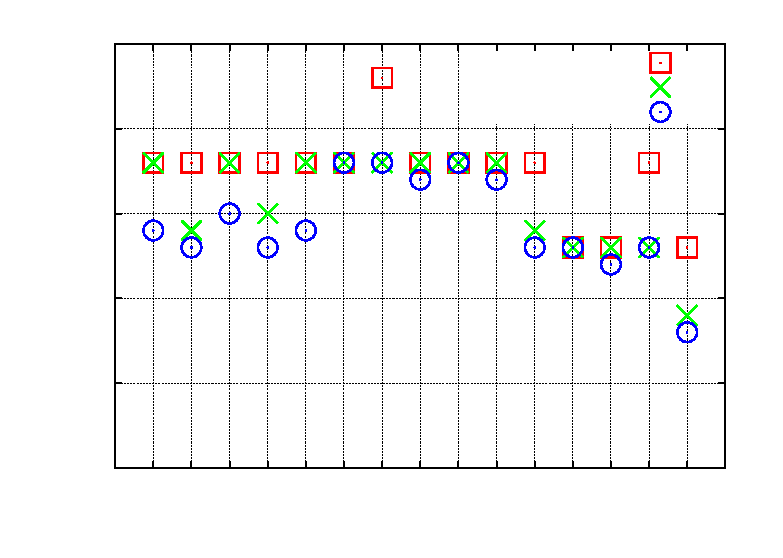
\includegraphics{../GNU/SelfTMitH}}%
    \gplfronttext
  \end{picture}%
\endgroup
}
    \caption{mit \(470 k\Omega\)}
    \label{fig:SelfTMitH}
  \end{subfigure}
  \caption{Selbsttest: Abweichung der Mittenspannung}
\end{figure}

\begin{figure}[H]
  \begin{subfigure}[b]{9cm}
  \centering
    \resizebox{9cm}{!}{% GNUPLOT: LaTeX picture with Postscript
\begingroup
  \makeatletter
  \providecommand\color[2][]{%
    \GenericError{(gnuplot) \space\space\space\@spaces}{%
      Package color not loaded in conjunction with
      terminal option `colourtext'%
    }{See the gnuplot documentation for explanation.%
    }{Either use 'blacktext' in gnuplot or load the package
      color.sty in LaTeX.}%
    \renewcommand\color[2][]{}%
  }%
  \providecommand\includegraphics[2][]{%
    \GenericError{(gnuplot) \space\space\space\@spaces}{%
      Package graphicx or graphics not loaded%
    }{See the gnuplot documentation for explanation.%
    }{The gnuplot epslatex terminal needs graphicx.sty or graphics.sty.}%
    \renewcommand\includegraphics[2][]{}%
  }%
  \providecommand\rotatebox[2]{#2}%
  \@ifundefined{ifGPcolor}{%
    \newif\ifGPcolor
    \GPcolortrue
  }{}%
  \@ifundefined{ifGPblacktext}{%
    \newif\ifGPblacktext
    \GPblacktexttrue
  }{}%
  % define a \g@addto@macro without @ in the name:
  \let\gplgaddtomacro\g@addto@macro
  % define empty templates for all commands taking text:
  \gdef\gplbacktext{}%
  \gdef\gplfronttext{}%
  \makeatother
  \ifGPblacktext
    % no textcolor at all
    \def\colorrgb#1{}%
    \def\colorgray#1{}%
  \else
    % gray or color?
    \ifGPcolor
      \def\colorrgb#1{\color[rgb]{#1}}%
      \def\colorgray#1{\color[gray]{#1}}%
      \expandafter\def\csname LTw\endcsname{\color{white}}%
      \expandafter\def\csname LTb\endcsname{\color{black}}%
      \expandafter\def\csname LTa\endcsname{\color{black}}%
      \expandafter\def\csname LT0\endcsname{\color[rgb]{1,0,0}}%
      \expandafter\def\csname LT1\endcsname{\color[rgb]{0,1,0}}%
      \expandafter\def\csname LT2\endcsname{\color[rgb]{0,0,1}}%
      \expandafter\def\csname LT3\endcsname{\color[rgb]{1,0,1}}%
      \expandafter\def\csname LT4\endcsname{\color[rgb]{0,1,1}}%
      \expandafter\def\csname LT5\endcsname{\color[rgb]{1,1,0}}%
      \expandafter\def\csname LT6\endcsname{\color[rgb]{0,0,0}}%
      \expandafter\def\csname LT7\endcsname{\color[rgb]{1,0.3,0}}%
      \expandafter\def\csname LT8\endcsname{\color[rgb]{0.5,0.5,0.5}}%
    \else
      % gray
      \def\colorrgb#1{\color{black}}%
      \def\colorgray#1{\color[gray]{#1}}%
      \expandafter\def\csname LTw\endcsname{\color{white}}%
      \expandafter\def\csname LTb\endcsname{\color{black}}%
      \expandafter\def\csname LTa\endcsname{\color{black}}%
      \expandafter\def\csname LT0\endcsname{\color{black}}%
      \expandafter\def\csname LT1\endcsname{\color{black}}%
      \expandafter\def\csname LT2\endcsname{\color{black}}%
      \expandafter\def\csname LT3\endcsname{\color{black}}%
      \expandafter\def\csname LT4\endcsname{\color{black}}%
      \expandafter\def\csname LT5\endcsname{\color{black}}%
      \expandafter\def\csname LT6\endcsname{\color{black}}%
      \expandafter\def\csname LT7\endcsname{\color{black}}%
      \expandafter\def\csname LT8\endcsname{\color{black}}%
    \fi
  \fi
  \setlength{\unitlength}{0.0500bp}%
  \begin{picture}(7200.00,5040.00)%
    \gplgaddtomacro\gplbacktext{%
      \csname LTb\endcsname%
      \put(682,704){\makebox(0,0)[r]{\strut{} 0}}%
      \csname LTb\endcsname%
      \put(682,1518){\makebox(0,0)[r]{\strut{} 1}}%
      \csname LTb\endcsname%
      \put(682,2332){\makebox(0,0)[r]{\strut{} 2}}%
      \csname LTb\endcsname%
      \put(682,3147){\makebox(0,0)[r]{\strut{} 3}}%
      \csname LTb\endcsname%
      \put(682,3961){\makebox(0,0)[r]{\strut{} 4}}%
      \csname LTb\endcsname%
      \put(682,4775){\makebox(0,0)[r]{\strut{} 5}}%
      \csname LTb\endcsname%
      \put(814,484){\makebox(0,0){\strut{} 0}}%
      \csname LTb\endcsname%
      \put(1188,484){\makebox(0,0){\strut{} 1}}%
      \csname LTb\endcsname%
      \put(1563,484){\makebox(0,0){\strut{} 2}}%
      \csname LTb\endcsname%
      \put(1937,484){\makebox(0,0){\strut{} 3}}%
      \csname LTb\endcsname%
      \put(2311,484){\makebox(0,0){\strut{} 4}}%
      \csname LTb\endcsname%
      \put(2686,484){\makebox(0,0){\strut{} 5}}%
      \csname LTb\endcsname%
      \put(3060,484){\makebox(0,0){\strut{} 6}}%
      \csname LTb\endcsname%
      \put(3434,484){\makebox(0,0){\strut{} 7}}%
      \csname LTb\endcsname%
      \put(3809,484){\makebox(0,0){\strut{} 8}}%
      \csname LTb\endcsname%
      \put(4183,484){\makebox(0,0){\strut{} 9}}%
      \csname LTb\endcsname%
      \put(4557,484){\makebox(0,0){\strut{} 10}}%
      \csname LTb\endcsname%
      \put(4931,484){\makebox(0,0){\strut{} 11}}%
      \csname LTb\endcsname%
      \put(5306,484){\makebox(0,0){\strut{} 12}}%
      \csname LTb\endcsname%
      \put(5680,484){\makebox(0,0){\strut{} 13}}%
      \csname LTb\endcsname%
      \put(6054,484){\makebox(0,0){\strut{} 14}}%
      \csname LTb\endcsname%
      \put(6429,484){\makebox(0,0){\strut{} 15}}%
      \csname LTb\endcsname%
      \put(6803,484){\makebox(0,0){\strut{} 16}}%
      \put(176,2739){\rotatebox{-270}{\makebox(0,0){\strut{}voltage / mV}}}%
      \put(3808,154){\makebox(0,0){\strut{}Processor number}}%
      \put(3808,4665){\makebox(0,0){\strut{}}}%
    }%
    \gplgaddtomacro\gplfronttext{%
      \csname LTb\endcsname%
      \put(5690,4594){\makebox(0,0)[r]{\strut{}RHbottom1}}%
      \csname LTb\endcsname%
      \put(5690,4358){\makebox(0,0)[r]{\strut{}RHbottom2}}%
      \csname LTb\endcsname%
      \put(5690,4122){\makebox(0,0)[r]{\strut{}RHbottom3}}%
    }%
    \gplbacktext
    \put(0,0){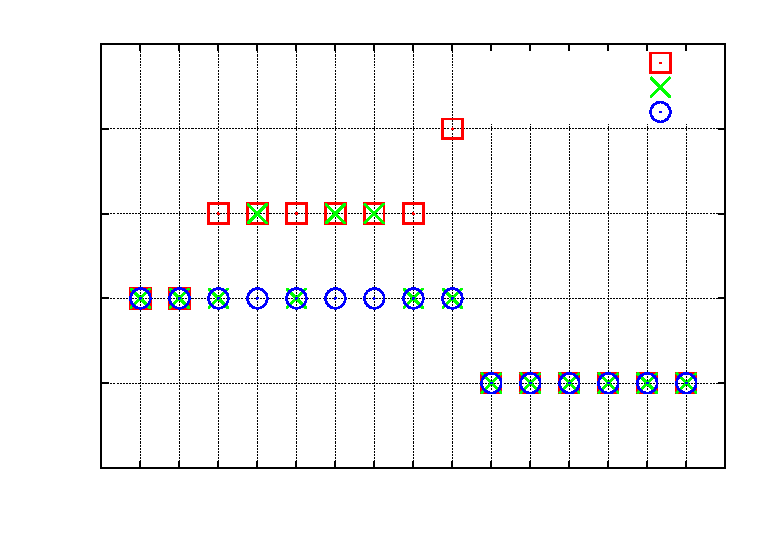
\includegraphics{../GNU/SelfTbottomH}}%
    \gplfronttext
  \end{picture}%
\endgroup
}
    \caption{mit \(470 k\Omega\) auf 0V}
    \label{fig:SelfTlowH}
  \end{subfigure}
  ~
  \begin{subfigure}[b]{9cm}
  \centering
    \resizebox{9cm}{!}{% GNUPLOT: LaTeX picture with Postscript
\begingroup
  \makeatletter
  \providecommand\color[2][]{%
    \GenericError{(gnuplot) \space\space\space\@spaces}{%
      Package color not loaded in conjunction with
      terminal option `colourtext'%
    }{See the gnuplot documentation for explanation.%
    }{Either use 'blacktext' in gnuplot or load the package
      color.sty in LaTeX.}%
    \renewcommand\color[2][]{}%
  }%
  \providecommand\includegraphics[2][]{%
    \GenericError{(gnuplot) \space\space\space\@spaces}{%
      Package graphicx or graphics not loaded%
    }{See the gnuplot documentation for explanation.%
    }{The gnuplot epslatex terminal needs graphicx.sty or graphics.sty.}%
    \renewcommand\includegraphics[2][]{}%
  }%
  \providecommand\rotatebox[2]{#2}%
  \@ifundefined{ifGPcolor}{%
    \newif\ifGPcolor
    \GPcolortrue
  }{}%
  \@ifundefined{ifGPblacktext}{%
    \newif\ifGPblacktext
    \GPblacktexttrue
  }{}%
  % define a \g@addto@macro without @ in the name:
  \let\gplgaddtomacro\g@addto@macro
  % define empty templates for all commands taking text:
  \gdef\gplbacktext{}%
  \gdef\gplfronttext{}%
  \makeatother
  \ifGPblacktext
    % no textcolor at all
    \def\colorrgb#1{}%
    \def\colorgray#1{}%
  \else
    % gray or color?
    \ifGPcolor
      \def\colorrgb#1{\color[rgb]{#1}}%
      \def\colorgray#1{\color[gray]{#1}}%
      \expandafter\def\csname LTw\endcsname{\color{white}}%
      \expandafter\def\csname LTb\endcsname{\color{black}}%
      \expandafter\def\csname LTa\endcsname{\color{black}}%
      \expandafter\def\csname LT0\endcsname{\color[rgb]{1,0,0}}%
      \expandafter\def\csname LT1\endcsname{\color[rgb]{0,1,0}}%
      \expandafter\def\csname LT2\endcsname{\color[rgb]{0,0,1}}%
      \expandafter\def\csname LT3\endcsname{\color[rgb]{1,0,1}}%
      \expandafter\def\csname LT4\endcsname{\color[rgb]{0,1,1}}%
      \expandafter\def\csname LT5\endcsname{\color[rgb]{1,1,0}}%
      \expandafter\def\csname LT6\endcsname{\color[rgb]{0,0,0}}%
      \expandafter\def\csname LT7\endcsname{\color[rgb]{1,0.3,0}}%
      \expandafter\def\csname LT8\endcsname{\color[rgb]{0.5,0.5,0.5}}%
    \else
      % gray
      \def\colorrgb#1{\color{black}}%
      \def\colorgray#1{\color[gray]{#1}}%
      \expandafter\def\csname LTw\endcsname{\color{white}}%
      \expandafter\def\csname LTb\endcsname{\color{black}}%
      \expandafter\def\csname LTa\endcsname{\color{black}}%
      \expandafter\def\csname LT0\endcsname{\color{black}}%
      \expandafter\def\csname LT1\endcsname{\color{black}}%
      \expandafter\def\csname LT2\endcsname{\color{black}}%
      \expandafter\def\csname LT3\endcsname{\color{black}}%
      \expandafter\def\csname LT4\endcsname{\color{black}}%
      \expandafter\def\csname LT5\endcsname{\color{black}}%
      \expandafter\def\csname LT6\endcsname{\color{black}}%
      \expandafter\def\csname LT7\endcsname{\color{black}}%
      \expandafter\def\csname LT8\endcsname{\color{black}}%
    \fi
  \fi
  \setlength{\unitlength}{0.0500bp}%
  \begin{picture}(7200.00,5040.00)%
    \gplgaddtomacro\gplbacktext{%
      \csname LTb\endcsname%
      \put(1078,704){\makebox(0,0)[r]{\strut{} 4996}}%
      \csname LTb\endcsname%
      \put(1078,1518){\makebox(0,0)[r]{\strut{} 4997}}%
      \csname LTb\endcsname%
      \put(1078,2332){\makebox(0,0)[r]{\strut{} 4998}}%
      \csname LTb\endcsname%
      \put(1078,3147){\makebox(0,0)[r]{\strut{} 4999}}%
      \csname LTb\endcsname%
      \put(1078,3961){\makebox(0,0)[r]{\strut{} 5000}}%
      \csname LTb\endcsname%
      \put(1078,4775){\makebox(0,0)[r]{\strut{} 5001}}%
      \csname LTb\endcsname%
      \put(1210,484){\makebox(0,0){\strut{} 0}}%
      \csname LTb\endcsname%
      \put(1560,484){\makebox(0,0){\strut{} 1}}%
      \csname LTb\endcsname%
      \put(1909,484){\makebox(0,0){\strut{} 2}}%
      \csname LTb\endcsname%
      \put(2259,484){\makebox(0,0){\strut{} 3}}%
      \csname LTb\endcsname%
      \put(2608,484){\makebox(0,0){\strut{} 4}}%
      \csname LTb\endcsname%
      \put(2958,484){\makebox(0,0){\strut{} 5}}%
      \csname LTb\endcsname%
      \put(3307,484){\makebox(0,0){\strut{} 6}}%
      \csname LTb\endcsname%
      \put(3657,484){\makebox(0,0){\strut{} 7}}%
      \csname LTb\endcsname%
      \put(4007,484){\makebox(0,0){\strut{} 8}}%
      \csname LTb\endcsname%
      \put(4356,484){\makebox(0,0){\strut{} 9}}%
      \csname LTb\endcsname%
      \put(4706,484){\makebox(0,0){\strut{} 10}}%
      \csname LTb\endcsname%
      \put(5055,484){\makebox(0,0){\strut{} 11}}%
      \csname LTb\endcsname%
      \put(5405,484){\makebox(0,0){\strut{} 12}}%
      \csname LTb\endcsname%
      \put(5754,484){\makebox(0,0){\strut{} 13}}%
      \csname LTb\endcsname%
      \put(6104,484){\makebox(0,0){\strut{} 14}}%
      \csname LTb\endcsname%
      \put(6453,484){\makebox(0,0){\strut{} 15}}%
      \csname LTb\endcsname%
      \put(6803,484){\makebox(0,0){\strut{} 16}}%
      \put(176,2739){\rotatebox{-270}{\makebox(0,0){\strut{}voltage / mV}}}%
      \put(4006,154){\makebox(0,0){\strut{}Processor number}}%
      \put(4006,4665){\makebox(0,0){\strut{}}}%
    }%
    \gplgaddtomacro\gplfronttext{%
      \csname LTb\endcsname%
      \put(5690,4594){\makebox(0,0)[r]{\strut{}RHtop1}}%
      \csname LTb\endcsname%
      \put(5690,4358){\makebox(0,0)[r]{\strut{}RHtop2}}%
      \csname LTb\endcsname%
      \put(5690,4122){\makebox(0,0)[r]{\strut{}RHtop3}}%
    }%
    \gplbacktext
    \put(0,0){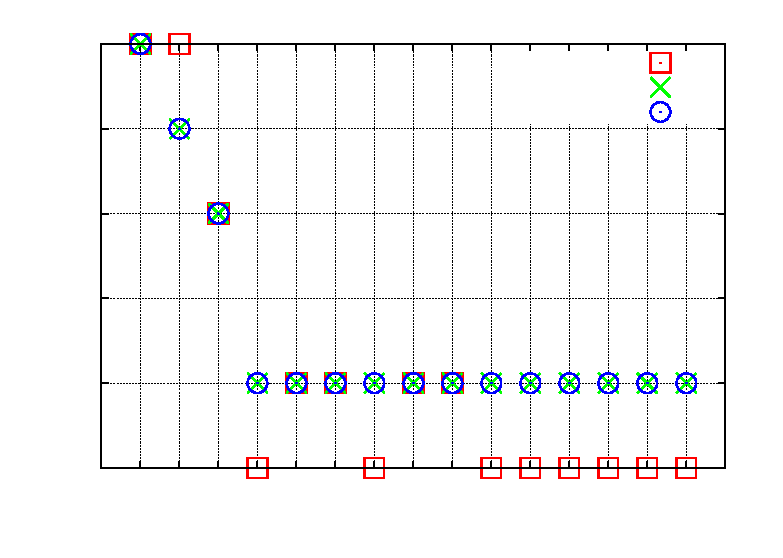
\includegraphics{../GNU/SelfTtopH}}%
    \gplfronttext
  \end{picture}%
\endgroup
}
    \caption{mit \(470 k\Omega\) auf 5V}
    \label{fig:SelfTtopH}
  \end{subfigure}
  \caption{Selbsttest: Eingangsspannung}
\end{figure}

\begin{figure}[H]
  \begin{subfigure}[b]{9cm}
  \centering
    \resizebox{9cm}{!}{% GNUPLOT: LaTeX picture with Postscript
\begingroup
  \makeatletter
  \providecommand\color[2][]{%
    \GenericError{(gnuplot) \space\space\space\@spaces}{%
      Package color not loaded in conjunction with
      terminal option `colourtext'%
    }{See the gnuplot documentation for explanation.%
    }{Either use 'blacktext' in gnuplot or load the package
      color.sty in LaTeX.}%
    \renewcommand\color[2][]{}%
  }%
  \providecommand\includegraphics[2][]{%
    \GenericError{(gnuplot) \space\space\space\@spaces}{%
      Package graphicx or graphics not loaded%
    }{See the gnuplot documentation for explanation.%
    }{The gnuplot epslatex terminal needs graphicx.sty or graphics.sty.}%
    \renewcommand\includegraphics[2][]{}%
  }%
  \providecommand\rotatebox[2]{#2}%
  \@ifundefined{ifGPcolor}{%
    \newif\ifGPcolor
    \GPcolortrue
  }{}%
  \@ifundefined{ifGPblacktext}{%
    \newif\ifGPblacktext
    \GPblacktexttrue
  }{}%
  % define a \g@addto@macro without @ in the name:
  \let\gplgaddtomacro\g@addto@macro
  % define empty templates for all commands taking text:
  \gdef\gplbacktext{}%
  \gdef\gplfronttext{}%
  \makeatother
  \ifGPblacktext
    % no textcolor at all
    \def\colorrgb#1{}%
    \def\colorgray#1{}%
  \else
    % gray or color?
    \ifGPcolor
      \def\colorrgb#1{\color[rgb]{#1}}%
      \def\colorgray#1{\color[gray]{#1}}%
      \expandafter\def\csname LTw\endcsname{\color{white}}%
      \expandafter\def\csname LTb\endcsname{\color{black}}%
      \expandafter\def\csname LTa\endcsname{\color{black}}%
      \expandafter\def\csname LT0\endcsname{\color[rgb]{1,0,0}}%
      \expandafter\def\csname LT1\endcsname{\color[rgb]{0,1,0}}%
      \expandafter\def\csname LT2\endcsname{\color[rgb]{0,0,1}}%
      \expandafter\def\csname LT3\endcsname{\color[rgb]{1,0,1}}%
      \expandafter\def\csname LT4\endcsname{\color[rgb]{0,1,1}}%
      \expandafter\def\csname LT5\endcsname{\color[rgb]{1,1,0}}%
      \expandafter\def\csname LT6\endcsname{\color[rgb]{0,0,0}}%
      \expandafter\def\csname LT7\endcsname{\color[rgb]{1,0.3,0}}%
      \expandafter\def\csname LT8\endcsname{\color[rgb]{0.5,0.5,0.5}}%
    \else
      % gray
      \def\colorrgb#1{\color{black}}%
      \def\colorgray#1{\color[gray]{#1}}%
      \expandafter\def\csname LTw\endcsname{\color{white}}%
      \expandafter\def\csname LTb\endcsname{\color{black}}%
      \expandafter\def\csname LTa\endcsname{\color{black}}%
      \expandafter\def\csname LT0\endcsname{\color{black}}%
      \expandafter\def\csname LT1\endcsname{\color{black}}%
      \expandafter\def\csname LT2\endcsname{\color{black}}%
      \expandafter\def\csname LT3\endcsname{\color{black}}%
      \expandafter\def\csname LT4\endcsname{\color{black}}%
      \expandafter\def\csname LT5\endcsname{\color{black}}%
      \expandafter\def\csname LT6\endcsname{\color{black}}%
      \expandafter\def\csname LT7\endcsname{\color{black}}%
      \expandafter\def\csname LT8\endcsname{\color{black}}%
    \fi
  \fi
  \setlength{\unitlength}{0.0500bp}%
  \begin{picture}(7200.00,5040.00)%
    \gplgaddtomacro\gplbacktext{%
      \csname LTb\endcsname%
      \put(946,704){\makebox(0,0)[r]{\strut{} 137}}%
      \csname LTb\endcsname%
      \put(946,1213){\makebox(0,0)[r]{\strut{} 138}}%
      \csname LTb\endcsname%
      \put(946,1722){\makebox(0,0)[r]{\strut{} 139}}%
      \csname LTb\endcsname%
      \put(946,2231){\makebox(0,0)[r]{\strut{} 140}}%
      \csname LTb\endcsname%
      \put(946,2740){\makebox(0,0)[r]{\strut{} 141}}%
      \csname LTb\endcsname%
      \put(946,3248){\makebox(0,0)[r]{\strut{} 142}}%
      \csname LTb\endcsname%
      \put(946,3757){\makebox(0,0)[r]{\strut{} 143}}%
      \csname LTb\endcsname%
      \put(946,4266){\makebox(0,0)[r]{\strut{} 144}}%
      \csname LTb\endcsname%
      \put(946,4775){\makebox(0,0)[r]{\strut{} 145}}%
      \csname LTb\endcsname%
      \put(1078,484){\makebox(0,0){\strut{} 0}}%
      \csname LTb\endcsname%
      \put(1436,484){\makebox(0,0){\strut{} 1}}%
      \csname LTb\endcsname%
      \put(1794,484){\makebox(0,0){\strut{} 2}}%
      \csname LTb\endcsname%
      \put(2151,484){\makebox(0,0){\strut{} 3}}%
      \csname LTb\endcsname%
      \put(2509,484){\makebox(0,0){\strut{} 4}}%
      \csname LTb\endcsname%
      \put(2867,484){\makebox(0,0){\strut{} 5}}%
      \csname LTb\endcsname%
      \put(3225,484){\makebox(0,0){\strut{} 6}}%
      \csname LTb\endcsname%
      \put(3583,484){\makebox(0,0){\strut{} 7}}%
      \csname LTb\endcsname%
      \put(3941,484){\makebox(0,0){\strut{} 8}}%
      \csname LTb\endcsname%
      \put(4298,484){\makebox(0,0){\strut{} 9}}%
      \csname LTb\endcsname%
      \put(4656,484){\makebox(0,0){\strut{} 10}}%
      \csname LTb\endcsname%
      \put(5014,484){\makebox(0,0){\strut{} 11}}%
      \csname LTb\endcsname%
      \put(5372,484){\makebox(0,0){\strut{} 12}}%
      \csname LTb\endcsname%
      \put(5730,484){\makebox(0,0){\strut{} 13}}%
      \csname LTb\endcsname%
      \put(6087,484){\makebox(0,0){\strut{} 14}}%
      \csname LTb\endcsname%
      \put(6445,484){\makebox(0,0){\strut{} 15}}%
      \csname LTb\endcsname%
      \put(6803,484){\makebox(0,0){\strut{} 16}}%
      \put(176,2739){\rotatebox{-270}{\makebox(0,0){\strut{}voltage / mV}}}%
      \put(3940,154){\makebox(0,0){\strut{}Processor number}}%
      \put(3940,4665){\makebox(0,0){\strut{}}}%
    }%
    \gplgaddtomacro\gplfronttext{%
      \csname LTb\endcsname%
      \put(5753,4602){\makebox(0,0)[r]{\strut{}RiLo1}}%
      \csname LTb\endcsname%
      \put(5753,4382){\makebox(0,0)[r]{\strut{}RiLo2}}%
      \csname LTb\endcsname%
      \put(5753,4162){\makebox(0,0)[r]{\strut{}RiLo3}}%
    }%
    \gplbacktext
    \put(0,0){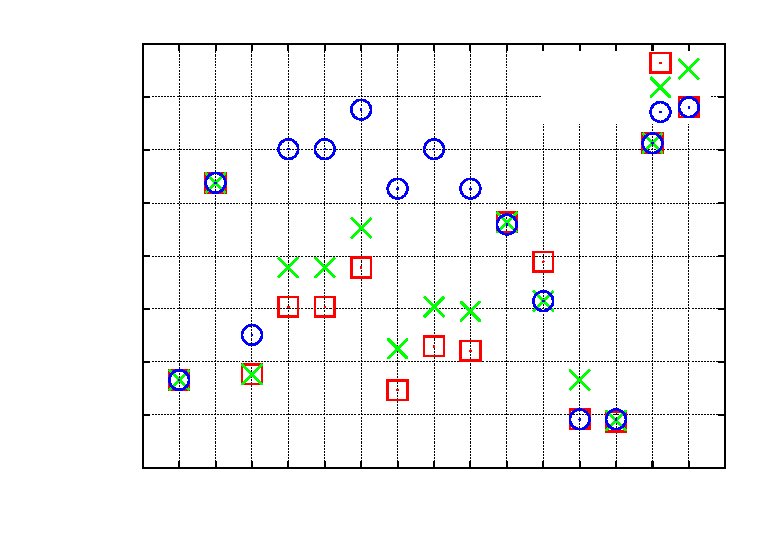
\includegraphics{../GNU/SelfTRiLo}}%
    \gplfronttext
  \end{picture}%
\endgroup
}
    \caption{mit \(680 \Omega\) auf 5V}
    \label{fig:SelfTRoL}
  \end{subfigure}
  ~
  \begin{subfigure}[b]{9cm}
  \centering
    \resizebox{9cm}{!}{% GNUPLOT: LaTeX picture with Postscript
\begingroup
  \makeatletter
  \providecommand\color[2][]{%
    \GenericError{(gnuplot) \space\space\space\@spaces}{%
      Package color not loaded in conjunction with
      terminal option `colourtext'%
    }{See the gnuplot documentation for explanation.%
    }{Either use 'blacktext' in gnuplot or load the package
      color.sty in LaTeX.}%
    \renewcommand\color[2][]{}%
  }%
  \providecommand\includegraphics[2][]{%
    \GenericError{(gnuplot) \space\space\space\@spaces}{%
      Package graphicx or graphics not loaded%
    }{See the gnuplot documentation for explanation.%
    }{The gnuplot epslatex terminal needs graphicx.sty or graphics.sty.}%
    \renewcommand\includegraphics[2][]{}%
  }%
  \providecommand\rotatebox[2]{#2}%
  \@ifundefined{ifGPcolor}{%
    \newif\ifGPcolor
    \GPcolortrue
  }{}%
  \@ifundefined{ifGPblacktext}{%
    \newif\ifGPblacktext
    \GPblacktexttrue
  }{}%
  % define a \g@addto@macro without @ in the name:
  \let\gplgaddtomacro\g@addto@macro
  % define empty templates for all commands taking text:
  \gdef\gplbacktext{}%
  \gdef\gplfronttext{}%
  \makeatother
  \ifGPblacktext
    % no textcolor at all
    \def\colorrgb#1{}%
    \def\colorgray#1{}%
  \else
    % gray or color?
    \ifGPcolor
      \def\colorrgb#1{\color[rgb]{#1}}%
      \def\colorgray#1{\color[gray]{#1}}%
      \expandafter\def\csname LTw\endcsname{\color{white}}%
      \expandafter\def\csname LTb\endcsname{\color{black}}%
      \expandafter\def\csname LTa\endcsname{\color{black}}%
      \expandafter\def\csname LT0\endcsname{\color[rgb]{1,0,0}}%
      \expandafter\def\csname LT1\endcsname{\color[rgb]{0,1,0}}%
      \expandafter\def\csname LT2\endcsname{\color[rgb]{0,0,1}}%
      \expandafter\def\csname LT3\endcsname{\color[rgb]{1,0,1}}%
      \expandafter\def\csname LT4\endcsname{\color[rgb]{0,1,1}}%
      \expandafter\def\csname LT5\endcsname{\color[rgb]{1,1,0}}%
      \expandafter\def\csname LT6\endcsname{\color[rgb]{0,0,0}}%
      \expandafter\def\csname LT7\endcsname{\color[rgb]{1,0.3,0}}%
      \expandafter\def\csname LT8\endcsname{\color[rgb]{0.5,0.5,0.5}}%
    \else
      % gray
      \def\colorrgb#1{\color{black}}%
      \def\colorgray#1{\color[gray]{#1}}%
      \expandafter\def\csname LTw\endcsname{\color{white}}%
      \expandafter\def\csname LTb\endcsname{\color{black}}%
      \expandafter\def\csname LTa\endcsname{\color{black}}%
      \expandafter\def\csname LT0\endcsname{\color{black}}%
      \expandafter\def\csname LT1\endcsname{\color{black}}%
      \expandafter\def\csname LT2\endcsname{\color{black}}%
      \expandafter\def\csname LT3\endcsname{\color{black}}%
      \expandafter\def\csname LT4\endcsname{\color{black}}%
      \expandafter\def\csname LT5\endcsname{\color{black}}%
      \expandafter\def\csname LT6\endcsname{\color{black}}%
      \expandafter\def\csname LT7\endcsname{\color{black}}%
      \expandafter\def\csname LT8\endcsname{\color{black}}%
    \fi
  \fi
  \setlength{\unitlength}{0.0500bp}%
  \begin{picture}(7200.00,5040.00)%
    \gplgaddtomacro\gplbacktext{%
      \csname LTb\endcsname%
      \put(946,704){\makebox(0,0)[r]{\strut{} 146}}%
      \csname LTb\endcsname%
      \put(946,1213){\makebox(0,0)[r]{\strut{} 148}}%
      \csname LTb\endcsname%
      \put(946,1722){\makebox(0,0)[r]{\strut{} 150}}%
      \csname LTb\endcsname%
      \put(946,2231){\makebox(0,0)[r]{\strut{} 152}}%
      \csname LTb\endcsname%
      \put(946,2740){\makebox(0,0)[r]{\strut{} 154}}%
      \csname LTb\endcsname%
      \put(946,3248){\makebox(0,0)[r]{\strut{} 156}}%
      \csname LTb\endcsname%
      \put(946,3757){\makebox(0,0)[r]{\strut{} 158}}%
      \csname LTb\endcsname%
      \put(946,4266){\makebox(0,0)[r]{\strut{} 160}}%
      \csname LTb\endcsname%
      \put(946,4775){\makebox(0,0)[r]{\strut{} 162}}%
      \csname LTb\endcsname%
      \put(1078,484){\makebox(0,0){\strut{} 0}}%
      \csname LTb\endcsname%
      \put(1436,484){\makebox(0,0){\strut{} 1}}%
      \csname LTb\endcsname%
      \put(1794,484){\makebox(0,0){\strut{} 2}}%
      \csname LTb\endcsname%
      \put(2151,484){\makebox(0,0){\strut{} 3}}%
      \csname LTb\endcsname%
      \put(2509,484){\makebox(0,0){\strut{} 4}}%
      \csname LTb\endcsname%
      \put(2867,484){\makebox(0,0){\strut{} 5}}%
      \csname LTb\endcsname%
      \put(3225,484){\makebox(0,0){\strut{} 6}}%
      \csname LTb\endcsname%
      \put(3583,484){\makebox(0,0){\strut{} 7}}%
      \csname LTb\endcsname%
      \put(3941,484){\makebox(0,0){\strut{} 8}}%
      \csname LTb\endcsname%
      \put(4298,484){\makebox(0,0){\strut{} 9}}%
      \csname LTb\endcsname%
      \put(4656,484){\makebox(0,0){\strut{} 10}}%
      \csname LTb\endcsname%
      \put(5014,484){\makebox(0,0){\strut{} 11}}%
      \csname LTb\endcsname%
      \put(5372,484){\makebox(0,0){\strut{} 12}}%
      \csname LTb\endcsname%
      \put(5730,484){\makebox(0,0){\strut{} 13}}%
      \csname LTb\endcsname%
      \put(6087,484){\makebox(0,0){\strut{} 14}}%
      \csname LTb\endcsname%
      \put(6445,484){\makebox(0,0){\strut{} 15}}%
      \csname LTb\endcsname%
      \put(6803,484){\makebox(0,0){\strut{} 16}}%
      \put(176,2739){\rotatebox{-270}{\makebox(0,0){\strut{}voltage / mV}}}%
      \put(3940,154){\makebox(0,0){\strut{}Processor number}}%
      \put(3940,4665){\makebox(0,0){\strut{}}}%
    }%
    \gplgaddtomacro\gplfronttext{%
      \csname LTb\endcsname%
      \put(5753,4602){\makebox(0,0)[r]{\strut{}RiHi1}}%
      \csname LTb\endcsname%
      \put(5753,4382){\makebox(0,0)[r]{\strut{}RiHi2}}%
      \csname LTb\endcsname%
      \put(5753,4162){\makebox(0,0)[r]{\strut{}RiHi3}}%
    }%
    \gplbacktext
    \put(0,0){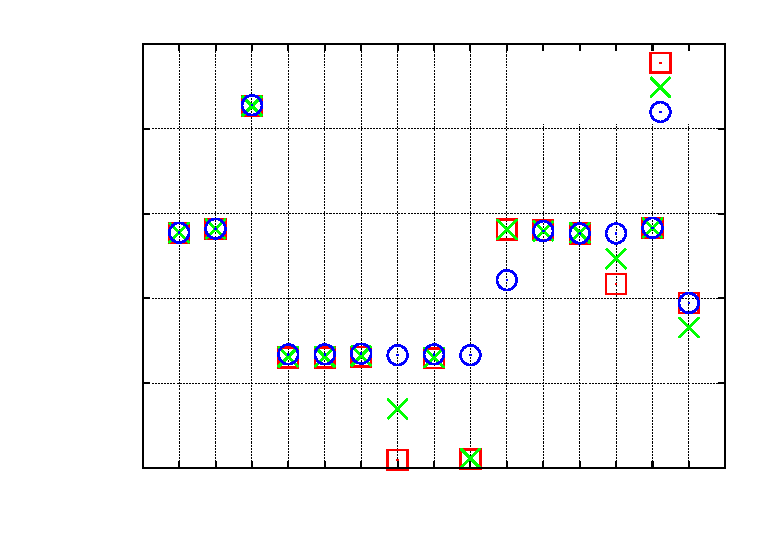
\includegraphics{../GNU/SelfTRiHi}}%
    \gplfronttext
  \end{picture}%
\endgroup
}
    \caption{mit \(680 \Omega\) auf 0V}
    \label{fig:SelfTRoH}
  \end{subfigure}
  \caption{Selbsttest: Ausgangswiderstand}
\end{figure}

\begin{figure}[H]
  \centering
  \resizebox{9cm}{!}{% GNUPLOT: LaTeX picture with Postscript
\begingroup
  \makeatletter
  \providecommand\color[2][]{%
    \GenericError{(gnuplot) \space\space\space\@spaces}{%
      Package color not loaded in conjunction with
      terminal option `colourtext'%
    }{See the gnuplot documentation for explanation.%
    }{Either use 'blacktext' in gnuplot or load the package
      color.sty in LaTeX.}%
    \renewcommand\color[2][]{}%
  }%
  \providecommand\includegraphics[2][]{%
    \GenericError{(gnuplot) \space\space\space\@spaces}{%
      Package graphicx or graphics not loaded%
    }{See the gnuplot documentation for explanation.%
    }{The gnuplot epslatex terminal needs graphicx.sty or graphics.sty.}%
    \renewcommand\includegraphics[2][]{}%
  }%
  \providecommand\rotatebox[2]{#2}%
  \@ifundefined{ifGPcolor}{%
    \newif\ifGPcolor
    \GPcolortrue
  }{}%
  \@ifundefined{ifGPblacktext}{%
    \newif\ifGPblacktext
    \GPblacktexttrue
  }{}%
  % define a \g@addto@macro without @ in the name:
  \let\gplgaddtomacro\g@addto@macro
  % define empty templates for all commands taking text:
  \gdef\gplbacktext{}%
  \gdef\gplfronttext{}%
  \makeatother
  \ifGPblacktext
    % no textcolor at all
    \def\colorrgb#1{}%
    \def\colorgray#1{}%
  \else
    % gray or color?
    \ifGPcolor
      \def\colorrgb#1{\color[rgb]{#1}}%
      \def\colorgray#1{\color[gray]{#1}}%
      \expandafter\def\csname LTw\endcsname{\color{white}}%
      \expandafter\def\csname LTb\endcsname{\color{black}}%
      \expandafter\def\csname LTa\endcsname{\color{black}}%
      \expandafter\def\csname LT0\endcsname{\color[rgb]{1,0,0}}%
      \expandafter\def\csname LT1\endcsname{\color[rgb]{0,1,0}}%
      \expandafter\def\csname LT2\endcsname{\color[rgb]{0,0,1}}%
      \expandafter\def\csname LT3\endcsname{\color[rgb]{1,0,1}}%
      \expandafter\def\csname LT4\endcsname{\color[rgb]{0,1,1}}%
      \expandafter\def\csname LT5\endcsname{\color[rgb]{1,1,0}}%
      \expandafter\def\csname LT6\endcsname{\color[rgb]{0,0,0}}%
      \expandafter\def\csname LT7\endcsname{\color[rgb]{1,0.3,0}}%
      \expandafter\def\csname LT8\endcsname{\color[rgb]{0.5,0.5,0.5}}%
    \else
      % gray
      \def\colorrgb#1{\color{black}}%
      \def\colorgray#1{\color[gray]{#1}}%
      \expandafter\def\csname LTw\endcsname{\color{white}}%
      \expandafter\def\csname LTb\endcsname{\color{black}}%
      \expandafter\def\csname LTa\endcsname{\color{black}}%
      \expandafter\def\csname LT0\endcsname{\color{black}}%
      \expandafter\def\csname LT1\endcsname{\color{black}}%
      \expandafter\def\csname LT2\endcsname{\color{black}}%
      \expandafter\def\csname LT3\endcsname{\color{black}}%
      \expandafter\def\csname LT4\endcsname{\color{black}}%
      \expandafter\def\csname LT5\endcsname{\color{black}}%
      \expandafter\def\csname LT6\endcsname{\color{black}}%
      \expandafter\def\csname LT7\endcsname{\color{black}}%
      \expandafter\def\csname LT8\endcsname{\color{black}}%
    \fi
  \fi
  \setlength{\unitlength}{0.0500bp}%
  \begin{picture}(7200.00,5040.00)%
    \gplgaddtomacro\gplbacktext{%
      \csname LTb\endcsname%
      \put(814,704){\makebox(0,0)[r]{\strut{} 36}}%
      \csname LTb\endcsname%
      \put(814,1286){\makebox(0,0)[r]{\strut{} 37}}%
      \csname LTb\endcsname%
      \put(814,1867){\makebox(0,0)[r]{\strut{} 38}}%
      \csname LTb\endcsname%
      \put(814,2449){\makebox(0,0)[r]{\strut{} 39}}%
      \csname LTb\endcsname%
      \put(814,3030){\makebox(0,0)[r]{\strut{} 40}}%
      \csname LTb\endcsname%
      \put(814,3612){\makebox(0,0)[r]{\strut{} 41}}%
      \csname LTb\endcsname%
      \put(814,4193){\makebox(0,0)[r]{\strut{} 42}}%
      \csname LTb\endcsname%
      \put(814,4775){\makebox(0,0)[r]{\strut{} 43}}%
      \csname LTb\endcsname%
      \put(946,484){\makebox(0,0){\strut{} 0}}%
      \csname LTb\endcsname%
      \put(1312,484){\makebox(0,0){\strut{} 1}}%
      \csname LTb\endcsname%
      \put(1678,484){\makebox(0,0){\strut{} 2}}%
      \csname LTb\endcsname%
      \put(2044,484){\makebox(0,0){\strut{} 3}}%
      \csname LTb\endcsname%
      \put(2410,484){\makebox(0,0){\strut{} 4}}%
      \csname LTb\endcsname%
      \put(2776,484){\makebox(0,0){\strut{} 5}}%
      \csname LTb\endcsname%
      \put(3142,484){\makebox(0,0){\strut{} 6}}%
      \csname LTb\endcsname%
      \put(3508,484){\makebox(0,0){\strut{} 7}}%
      \csname LTb\endcsname%
      \put(3875,484){\makebox(0,0){\strut{} 8}}%
      \csname LTb\endcsname%
      \put(4241,484){\makebox(0,0){\strut{} 9}}%
      \csname LTb\endcsname%
      \put(4607,484){\makebox(0,0){\strut{} 10}}%
      \csname LTb\endcsname%
      \put(4973,484){\makebox(0,0){\strut{} 11}}%
      \csname LTb\endcsname%
      \put(5339,484){\makebox(0,0){\strut{} 12}}%
      \csname LTb\endcsname%
      \put(5705,484){\makebox(0,0){\strut{} 13}}%
      \csname LTb\endcsname%
      \put(6071,484){\makebox(0,0){\strut{} 14}}%
      \csname LTb\endcsname%
      \put(6437,484){\makebox(0,0){\strut{} 15}}%
      \csname LTb\endcsname%
      \put(6803,484){\makebox(0,0){\strut{} 16}}%
      \put(176,2739){\rotatebox{-270}{\makebox(0,0){\strut{}Capacity / pF}}}%
      \put(3874,154){\makebox(0,0){\strut{}Processor number}}%
      \put(3874,4665){\makebox(0,0){\strut{}}}%
    }%
    \gplgaddtomacro\gplfronttext{%
      \csname LTb\endcsname%
      \put(5690,4594){\makebox(0,0)[r]{\strut{}CNULL1}}%
      \csname LTb\endcsname%
      \put(5690,4358){\makebox(0,0)[r]{\strut{}CNULL2}}%
      \csname LTb\endcsname%
      \put(5690,4122){\makebox(0,0)[r]{\strut{}CNULL3}}%
    }%
    \gplbacktext
    \put(0,0){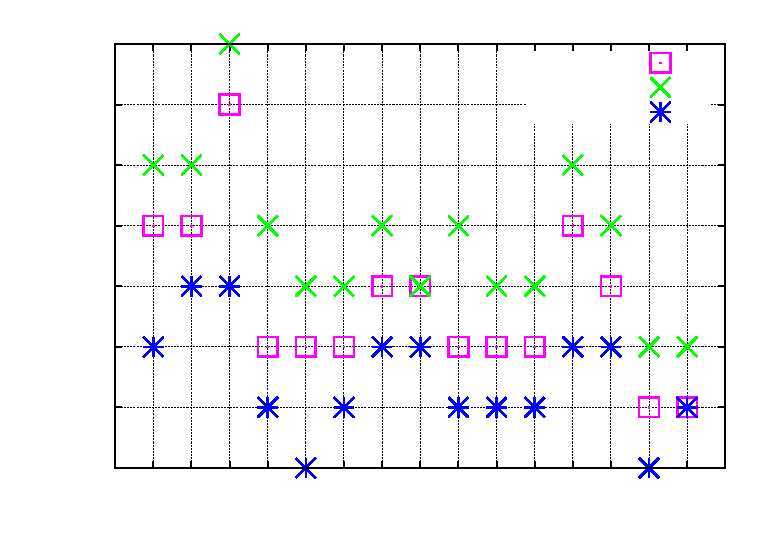
\includegraphics{../GNU/SelfTcap0}}%
    \gplfronttext
  \end{picture}%
\endgroup
}
  \caption{Selbsttest: Nullwert der Kapazitätsmessung}
  \label{fig:SelfTcap}
\end{figure}

\begin{figure}[H]
  \centering
  \resizebox{9cm}{!}{% GNUPLOT: LaTeX picture with Postscript
\begingroup
  \makeatletter
  \providecommand\color[2][]{%
    \GenericError{(gnuplot) \space\space\space\@spaces}{%
      Package color not loaded in conjunction with
      terminal option `colourtext'%
    }{See the gnuplot documentation for explanation.%
    }{Either use 'blacktext' in gnuplot or load the package
      color.sty in LaTeX.}%
    \renewcommand\color[2][]{}%
  }%
  \providecommand\includegraphics[2][]{%
    \GenericError{(gnuplot) \space\space\space\@spaces}{%
      Package graphicx or graphics not loaded%
    }{See the gnuplot documentation for explanation.%
    }{The gnuplot epslatex terminal needs graphicx.sty or graphics.sty.}%
    \renewcommand\includegraphics[2][]{}%
  }%
  \providecommand\rotatebox[2]{#2}%
  \@ifundefined{ifGPcolor}{%
    \newif\ifGPcolor
    \GPcolortrue
  }{}%
  \@ifundefined{ifGPblacktext}{%
    \newif\ifGPblacktext
    \GPblacktexttrue
  }{}%
  % define a \g@addto@macro without @ in the name:
  \let\gplgaddtomacro\g@addto@macro
  % define empty templates for all commands taking text:
  \gdef\gplbacktext{}%
  \gdef\gplfronttext{}%
  \makeatother
  \ifGPblacktext
    % no textcolor at all
    \def\colorrgb#1{}%
    \def\colorgray#1{}%
  \else
    % gray or color?
    \ifGPcolor
      \def\colorrgb#1{\color[rgb]{#1}}%
      \def\colorgray#1{\color[gray]{#1}}%
      \expandafter\def\csname LTw\endcsname{\color{white}}%
      \expandafter\def\csname LTb\endcsname{\color{black}}%
      \expandafter\def\csname LTa\endcsname{\color{black}}%
      \expandafter\def\csname LT0\endcsname{\color[rgb]{1,0,0}}%
      \expandafter\def\csname LT1\endcsname{\color[rgb]{0,1,0}}%
      \expandafter\def\csname LT2\endcsname{\color[rgb]{0,0,1}}%
      \expandafter\def\csname LT3\endcsname{\color[rgb]{1,0,1}}%
      \expandafter\def\csname LT4\endcsname{\color[rgb]{0,1,1}}%
      \expandafter\def\csname LT5\endcsname{\color[rgb]{1,1,0}}%
      \expandafter\def\csname LT6\endcsname{\color[rgb]{0,0,0}}%
      \expandafter\def\csname LT7\endcsname{\color[rgb]{1,0.3,0}}%
      \expandafter\def\csname LT8\endcsname{\color[rgb]{0.5,0.5,0.5}}%
    \else
      % gray
      \def\colorrgb#1{\color{black}}%
      \def\colorgray#1{\color[gray]{#1}}%
      \expandafter\def\csname LTw\endcsname{\color{white}}%
      \expandafter\def\csname LTb\endcsname{\color{black}}%
      \expandafter\def\csname LTa\endcsname{\color{black}}%
      \expandafter\def\csname LT0\endcsname{\color{black}}%
      \expandafter\def\csname LT1\endcsname{\color{black}}%
      \expandafter\def\csname LT2\endcsname{\color{black}}%
      \expandafter\def\csname LT3\endcsname{\color{black}}%
      \expandafter\def\csname LT4\endcsname{\color{black}}%
      \expandafter\def\csname LT5\endcsname{\color{black}}%
      \expandafter\def\csname LT6\endcsname{\color{black}}%
      \expandafter\def\csname LT7\endcsname{\color{black}}%
      \expandafter\def\csname LT8\endcsname{\color{black}}%
    \fi
  \fi
  \setlength{\unitlength}{0.0500bp}%
  \begin{picture}(7200.00,5040.00)%
    \gplgaddtomacro\gplbacktext{%
      \csname LTb\endcsname%
      \put(814,704){\makebox(0,0)[r]{\strut{}-60}}%
      \csname LTb\endcsname%
      \put(814,1286){\makebox(0,0)[r]{\strut{}-40}}%
      \csname LTb\endcsname%
      \put(814,1867){\makebox(0,0)[r]{\strut{}-20}}%
      \csname LTb\endcsname%
      \put(814,2449){\makebox(0,0)[r]{\strut{} 0}}%
      \csname LTb\endcsname%
      \put(814,3030){\makebox(0,0)[r]{\strut{} 20}}%
      \csname LTb\endcsname%
      \put(814,3612){\makebox(0,0)[r]{\strut{} 40}}%
      \csname LTb\endcsname%
      \put(814,4193){\makebox(0,0)[r]{\strut{} 60}}%
      \csname LTb\endcsname%
      \put(814,4775){\makebox(0,0)[r]{\strut{} 80}}%
      \csname LTb\endcsname%
      \put(946,484){\makebox(0,0){\strut{} 0}}%
      \csname LTb\endcsname%
      \put(1312,484){\makebox(0,0){\strut{} 1}}%
      \csname LTb\endcsname%
      \put(1678,484){\makebox(0,0){\strut{} 2}}%
      \csname LTb\endcsname%
      \put(2044,484){\makebox(0,0){\strut{} 3}}%
      \csname LTb\endcsname%
      \put(2410,484){\makebox(0,0){\strut{} 4}}%
      \csname LTb\endcsname%
      \put(2776,484){\makebox(0,0){\strut{} 5}}%
      \csname LTb\endcsname%
      \put(3142,484){\makebox(0,0){\strut{} 6}}%
      \csname LTb\endcsname%
      \put(3508,484){\makebox(0,0){\strut{} 7}}%
      \csname LTb\endcsname%
      \put(3875,484){\makebox(0,0){\strut{} 8}}%
      \csname LTb\endcsname%
      \put(4241,484){\makebox(0,0){\strut{} 9}}%
      \csname LTb\endcsname%
      \put(4607,484){\makebox(0,0){\strut{} 10}}%
      \csname LTb\endcsname%
      \put(4973,484){\makebox(0,0){\strut{} 11}}%
      \csname LTb\endcsname%
      \put(5339,484){\makebox(0,0){\strut{} 12}}%
      \csname LTb\endcsname%
      \put(5705,484){\makebox(0,0){\strut{} 13}}%
      \csname LTb\endcsname%
      \put(6071,484){\makebox(0,0){\strut{} 14}}%
      \csname LTb\endcsname%
      \put(6437,484){\makebox(0,0){\strut{} 15}}%
      \csname LTb\endcsname%
      \put(6803,484){\makebox(0,0){\strut{} 16}}%
      \put(176,2739){\rotatebox{-270}{\makebox(0,0){\strut{}Voltage correction / mV}}}%
      \put(3874,154){\makebox(0,0){\strut{}Processor number}}%
      \put(3874,4665){\makebox(0,0){\strut{}}}%
    }%
    \gplgaddtomacro\gplfronttext{%
      \csname LTb\endcsname%
      \put(5690,4594){\makebox(0,0)[r]{\strut{}REF\_C\_KORR}}%
      \csname LTb\endcsname%
      \put(5690,4358){\makebox(0,0)[r]{\strut{}REF\_R\_KORR}}%
    }%
    \gplbacktext
    \put(0,0){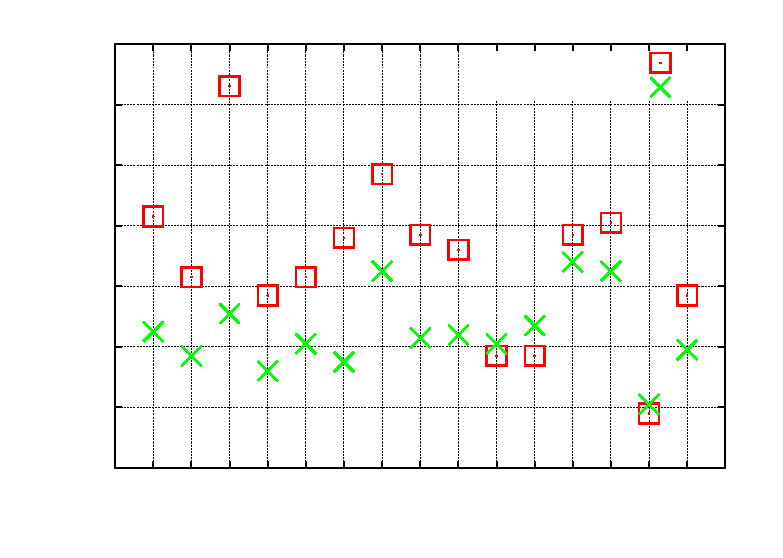
\includegraphics{../GNU/SelfTrefKorr}}%
    \gplfronttext
  \end{picture}%
\endgroup
}
  \caption{Selbsttest: Korrekturwerte nach automatischer Kalibration}
  \label{fig:SelfTrefKorr}
\end{figure}

Zuletzt möchte ich die Differenzen der am AREF-Pin mit einem Multimeter
gemessenen Spannungen und der intern mit dem ADC gemessenen Referenzspannungen der
15 verschiedenen ATmegas und die mit dem automatischen Abgleich
gefundenen Korrekturspannung (REF\_R\_KORR) in Abbildung~\ref{fig:SelfTrefDiff} gegenüberstellen.
Sie können sehen, dass die Werte der automatischen Kalibration nahezu den extern
gemessenen Referenz-Spannungswerten folgen.

\begin{figure}[H]
  \centering
  \resizebox{9cm}{!}{% GNUPLOT: LaTeX picture with Postscript
\begingroup
  \makeatletter
  \providecommand\color[2][]{%
    \GenericError{(gnuplot) \space\space\space\@spaces}{%
      Package color not loaded in conjunction with
      terminal option `colourtext'%
    }{See the gnuplot documentation for explanation.%
    }{Either use 'blacktext' in gnuplot or load the package
      color.sty in LaTeX.}%
    \renewcommand\color[2][]{}%
  }%
  \providecommand\includegraphics[2][]{%
    \GenericError{(gnuplot) \space\space\space\@spaces}{%
      Package graphicx or graphics not loaded%
    }{See the gnuplot documentation for explanation.%
    }{The gnuplot epslatex terminal needs graphicx.sty or graphics.sty.}%
    \renewcommand\includegraphics[2][]{}%
  }%
  \providecommand\rotatebox[2]{#2}%
  \@ifundefined{ifGPcolor}{%
    \newif\ifGPcolor
    \GPcolortrue
  }{}%
  \@ifundefined{ifGPblacktext}{%
    \newif\ifGPblacktext
    \GPblacktexttrue
  }{}%
  % define a \g@addto@macro without @ in the name:
  \let\gplgaddtomacro\g@addto@macro
  % define empty templates for all commands taking text:
  \gdef\gplbacktext{}%
  \gdef\gplfronttext{}%
  \makeatother
  \ifGPblacktext
    % no textcolor at all
    \def\colorrgb#1{}%
    \def\colorgray#1{}%
  \else
    % gray or color?
    \ifGPcolor
      \def\colorrgb#1{\color[rgb]{#1}}%
      \def\colorgray#1{\color[gray]{#1}}%
      \expandafter\def\csname LTw\endcsname{\color{white}}%
      \expandafter\def\csname LTb\endcsname{\color{black}}%
      \expandafter\def\csname LTa\endcsname{\color{black}}%
      \expandafter\def\csname LT0\endcsname{\color[rgb]{1,0,0}}%
      \expandafter\def\csname LT1\endcsname{\color[rgb]{0,1,0}}%
      \expandafter\def\csname LT2\endcsname{\color[rgb]{0,0,1}}%
      \expandafter\def\csname LT3\endcsname{\color[rgb]{1,0,1}}%
      \expandafter\def\csname LT4\endcsname{\color[rgb]{0,1,1}}%
      \expandafter\def\csname LT5\endcsname{\color[rgb]{1,1,0}}%
      \expandafter\def\csname LT6\endcsname{\color[rgb]{0,0,0}}%
      \expandafter\def\csname LT7\endcsname{\color[rgb]{1,0.3,0}}%
      \expandafter\def\csname LT8\endcsname{\color[rgb]{0.5,0.5,0.5}}%
    \else
      % gray
      \def\colorrgb#1{\color{black}}%
      \def\colorgray#1{\color[gray]{#1}}%
      \expandafter\def\csname LTw\endcsname{\color{white}}%
      \expandafter\def\csname LTb\endcsname{\color{black}}%
      \expandafter\def\csname LTa\endcsname{\color{black}}%
      \expandafter\def\csname LT0\endcsname{\color{black}}%
      \expandafter\def\csname LT1\endcsname{\color{black}}%
      \expandafter\def\csname LT2\endcsname{\color{black}}%
      \expandafter\def\csname LT3\endcsname{\color{black}}%
      \expandafter\def\csname LT4\endcsname{\color{black}}%
      \expandafter\def\csname LT5\endcsname{\color{black}}%
      \expandafter\def\csname LT6\endcsname{\color{black}}%
      \expandafter\def\csname LT7\endcsname{\color{black}}%
      \expandafter\def\csname LT8\endcsname{\color{black}}%
    \fi
  \fi
  \setlength{\unitlength}{0.0500bp}%
  \begin{picture}(7200.00,5040.00)%
    \gplgaddtomacro\gplbacktext{%
      \csname LTb\endcsname%
      \put(814,704){\makebox(0,0)[r]{\strut{}-40}}%
      \csname LTb\endcsname%
      \put(814,1213){\makebox(0,0)[r]{\strut{}-30}}%
      \csname LTb\endcsname%
      \put(814,1722){\makebox(0,0)[r]{\strut{}-20}}%
      \csname LTb\endcsname%
      \put(814,2231){\makebox(0,0)[r]{\strut{}-10}}%
      \csname LTb\endcsname%
      \put(814,2740){\makebox(0,0)[r]{\strut{} 0}}%
      \csname LTb\endcsname%
      \put(814,3248){\makebox(0,0)[r]{\strut{} 10}}%
      \csname LTb\endcsname%
      \put(814,3757){\makebox(0,0)[r]{\strut{} 20}}%
      \csname LTb\endcsname%
      \put(814,4266){\makebox(0,0)[r]{\strut{} 30}}%
      \csname LTb\endcsname%
      \put(814,4775){\makebox(0,0)[r]{\strut{} 40}}%
      \csname LTb\endcsname%
      \put(946,484){\makebox(0,0){\strut{} 0}}%
      \csname LTb\endcsname%
      \put(1312,484){\makebox(0,0){\strut{} 1}}%
      \csname LTb\endcsname%
      \put(1678,484){\makebox(0,0){\strut{} 2}}%
      \csname LTb\endcsname%
      \put(2044,484){\makebox(0,0){\strut{} 3}}%
      \csname LTb\endcsname%
      \put(2410,484){\makebox(0,0){\strut{} 4}}%
      \csname LTb\endcsname%
      \put(2776,484){\makebox(0,0){\strut{} 5}}%
      \csname LTb\endcsname%
      \put(3142,484){\makebox(0,0){\strut{} 6}}%
      \csname LTb\endcsname%
      \put(3508,484){\makebox(0,0){\strut{} 7}}%
      \csname LTb\endcsname%
      \put(3875,484){\makebox(0,0){\strut{} 8}}%
      \csname LTb\endcsname%
      \put(4241,484){\makebox(0,0){\strut{} 9}}%
      \csname LTb\endcsname%
      \put(4607,484){\makebox(0,0){\strut{} 10}}%
      \csname LTb\endcsname%
      \put(4973,484){\makebox(0,0){\strut{} 11}}%
      \csname LTb\endcsname%
      \put(5339,484){\makebox(0,0){\strut{} 12}}%
      \csname LTb\endcsname%
      \put(5705,484){\makebox(0,0){\strut{} 13}}%
      \csname LTb\endcsname%
      \put(6071,484){\makebox(0,0){\strut{} 14}}%
      \csname LTb\endcsname%
      \put(6437,484){\makebox(0,0){\strut{} 15}}%
      \csname LTb\endcsname%
      \put(6803,484){\makebox(0,0){\strut{} 16}}%
      \put(176,2739){\rotatebox{-270}{\makebox(0,0){\strut{}Voltage difference / mV}}}%
      \put(3874,154){\makebox(0,0){\strut{}Processor number}}%
      \put(3874,4665){\makebox(0,0){\strut{}}}%
    }%
    \gplgaddtomacro\gplfronttext{%
      \csname LTb\endcsname%
      \put(5690,4594){\makebox(0,0)[r]{\strut{}AREF - REF}}%
      \csname LTb\endcsname%
      \put(5690,4358){\makebox(0,0)[r]{\strut{}REF\_R\_KORR}}%
    }%
    \gplbacktext
    \put(0,0){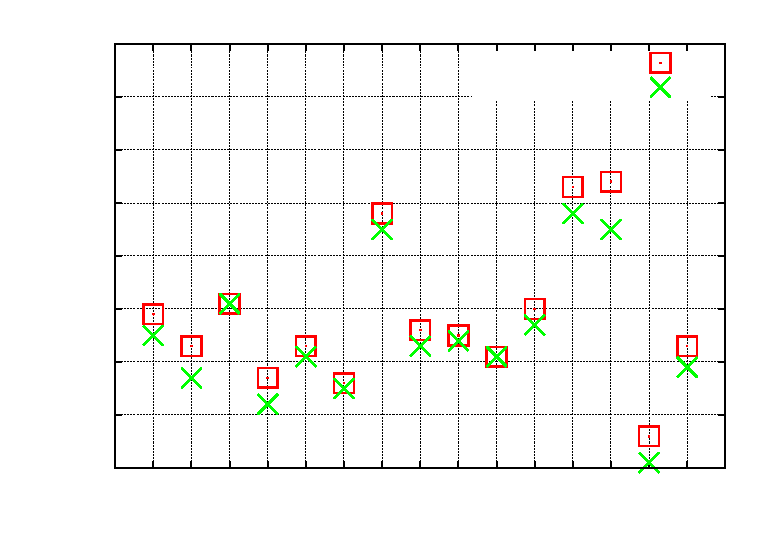
\includegraphics{../GNU/SelfTrefDiff}}%
    \gplfronttext
  \end{picture}%
\endgroup
}
  \caption{Selbsttest: Spannungsdifferenz der internen Referenz}
  \label{fig:SelfTrefDiff}
\end{figure}

